\documentclass[12pt,a4paper]{article}
\usepackage[utf8]{inputenc}
\usepackage[french]{babel}
\usepackage{geometry}
\usepackage{graphicx}
\usepackage{hyperref}
\usepackage{amsmath}
\usepackage{amsfonts}
\usepackage{amssymb}
\usepackage{booktabs}
\usepackage{array}
\usepackage{longtable}
\usepackage{listings}
\usepackage{xcolor}
\usepackage{fancyhdr}
\usepackage{titlesec}
\usepackage{enumitem}
\usepackage{float}
\usepackage{caption}
\usepackage{subcaption}
\usepackage{url}
\usepackage{listings}
\usepackage{color}
\usepackage{tcolorbox}
\usepackage{changepage}
\usepackage{afterpage}

% Load global configuration

%=== File containing Global Configuration of the report ===%
%                                                          %
% Copyright (C) ISI - All Rights Reserved                  %
% Proprietary                                              %
% Written by Med Hossam <med.hossam@gmail.com>, April 2016 %
%                                                          %
% @author: HEDHILI Med Houssemeddine                       %
% @linkedin: http://tn.linkedin.com/in/medhossam           %
%==========================================================%

%=========== You MUST type your information here ==========%
% global_config.tex file is designed to configure your     %
% cover pages (main, back and black covers)                %
%==========================================================%

%============= Config new columns type ==============%
\newcolumntype{L}{>{\raggedright\arraybackslash}}
\newcolumntype{R}{>{\raggedleft\arraybackslash}}
\newcolumntype{C}{>{\centering\arraybackslash}}
%==================================================%

%========= Config the cover section ==========%

\title{Conception et Développement d'une Plateforme Web d'Analyse Financière Basée sur l'Architecture Medallion ETL pour la Bourse des Valeurs Mobilières de Tunis (BVMT)}

\author{BACCA}
%%% if necessary
% Set isBinomal to true and type second author name
%\setboolean{isBinomal}{true}
%\secondAuthor{Prénom NOM}

\diplomaName{Diplôme National d'Ingénieur en Sciences Appliquées et Technologiques}
\speciality{Génie Informatique}
%\speciality{Génie des Télécommunications et Réseaux}
%\speciality{Génie Informatique des Systèmes Industriels}

%% Encadrant professionnel
\proFramerName{Monsieur [Nom de l'Encadrant Professionnel]}
\proFramerSpeciality{Ingénieur Informatique}

%% Encadrant académique
\academicFramerName{Monsieur [Nom de l'Encadrant Académique]}
\academicFramerSpeciality{Maître de Conférences}

%% Entreprise d'accueil
\companyName{Institut Supérieur d'Informatique (ISI)}

%% Année universitaire
\collegeYear{2024 - 2025}

%%%%%% Signatures section %%%%%%

% You can simply remove theses sentences by typing an empty string
% \proSignSentence{}

\proSignSentence{J'autorise l'étudiant à faire le dépôt de son rapport de stage en vue d'une soutenance.}

\academicSignSentence{J'autorise l'étudiant à faire le dépôt de son rapport de stage en vue d'une soutenance.}

%%% FR
\frenchAbstract{Ce projet présente la conception et le développement d'une plateforme web complète d'analyse financière pour la Bourse des Valeurs Mobilières de Tunis (BVMT). L'architecture repose sur le modèle Medallion ETL avec quatre couches distinctes (Bronze, Silver, Golden, Diamond) permettant une transformation progressive des données financières brutes en insights analytiques avancés. La plateforme intègre un système de scraping automatisé, un pipeline ETL robuste, des tableaux de bord Power BI, et un chatbot IA spécialisé. Développée selon la méthodologie Scrum, cette solution offre une approche moderne et évolutive pour l'analyse des marchés financiers tunisiens.}

\frenchAbstractKeywords{ETL, Medallion Architecture, BVMT, Scraping, Power BI, Chatbot IA, Scrum, Analyse Financière}

%%% EN
\englishAbstract{This project presents the design and development of a comprehensive web platform for financial analysis of the Tunisian Stock Exchange (BVMT). The architecture is based on the Medallion ETL model with four distinct layers (Bronze, Silver, Golden, Diamond) enabling progressive transformation of raw financial data into advanced analytical insights. The platform integrates an automated scraping system, a robust ETL pipeline, Power BI dashboards, and a specialized AI chatbot. Developed using Scrum methodology, this solution offers a modern and scalable approach for analyzing Tunisian financial markets.}

\englishAbstractKeywords{ETL, Medallion Architecture, BVMT, Scraping, Power BI, AI Chatbot, Scrum, Financial Analysis}

%% if you want to get rid of the company address just set the boolean variable to false
% PS : it's optional
\setboolean{wantToTypeCompanyAddress}{false}

\companyEmail{contact@isi.rnu.tn}
\companyTel{71 111 111}
\companyFax{71 222 222}
\companyAddressAR{نهج بحيرة ملاران - ضفاف البحيرة - تونس}
\companyAddressFR{Rue du Lac Malaren, Les Berges du Lac 1053 Tunis}

% Page setup
\geometry{margin=2.5cm}
\pagestyle{fancy}
\fancyhf{}
\fancyhead[L]{\leftmark}
\fancyhead[R]{\thepage}
\renewcommand{\headrulewidth}{0.4pt}

% Title formatting
\titleformat{\section}{\Large\bfseries}{\thesection}{1em}{}
\titleformat{\subsection}{\large\bfseries}{\thesubsection}{1em}{}
\titleformat{\subsubsection}{\normalsize\bfseries}{\thesubsubsection}{1em}{}

% Code listing setup
\lstset{
    language=Python,
    basicstyle=\ttfamily\small,
    keywordstyle=\color{blue},
    commentstyle=\color{green!60!black},
    stringstyle=\color{red},
    numbers=left,
    numberstyle=\tiny,
    numbersep=5pt,
    frame=single,
    breaklines=true,
    showstringspaces=false
}

% Hyperref setup
\hypersetup{
    colorlinks=true,
    linkcolor=blue,
    filecolor=magenta,
    urlcolor=cyan,
    citecolor=red
}

% Custom commands
\newcommand{\blankpage}{\newpage\thispagestyle{empty}\null\newpage}

% Image width command for consistent sizing
\newcommand{\figwidth}{0.5\textwidth}

\begin{document}

% Title page
%== It's advised to not modify the content of this file ===%
% To set your information, go to global_config.tex file    %
%==========================================================%

\thispagestyle{cover}%
\newgeometry{bottom=25mm,left=20mm,top=15mm,right=20mm}
\hspace{-47pt}
\begin{minipage}[l]{0.2\columnwidth}
\vspace{6mm}

\includegraphics[width=1.1\columnwidth]{img/tekup.png}\\
\end{minipage}
\hfill
\begin{minipage}[l]{0.6\columnwidth}
\centering
\footnotesize
\textbf{{République Tunisienne}}\\
\vspace{1.5mm}
\textbf{{Ministère de l'Enseignement Supérieur\\
et de la Recherche Scientifique}}\\
\vspace{1.5mm}
%\textbf{{Université de Tunis El Manar}}\\
\vspace{1.5mm}
\textbf{{École Supérieur Privée d'ingénierie et de technologie}}\\
\vspace{1.5mm}
\textbf{{TEK-UP}}\\
\vspace{1.5mm}
\end{minipage}
\hfill
\begin{minipage}[l]{0.02\columnwidth}
\end{minipage}
\hfill
\begin{minipage}[l]{0.2\columnwidth}
\vspace{6mm}

\includegraphics[width=1.3\columnwidth]{img/bvmt logo.png}\\
\end{minipage}
\vskip1.5cm

\begin{center}
{\LARGE{\textbf{\textsc{Rapport de Projet de Fin d'Études}}}}\\
\vskip0.5cm
\large

{\textbf{Présenté en vue de l'obtention du}}\\
\vskip2mm
{\textbf{\@diplomaName}}\\
{\textbf{Spécialité : \@speciality}}\\
{}
\end{center}

\begin{center}
\textrm{Réalisé par}\\
MAHDI BACCAR
\vskip12mm

\definecolor{isiBlue}{RGB}{31, 78, 121}

\begin{changemargin}{-9mm}{0cm}
\begin{minipage}[l]{1.1\columnwidth}
\begin{tcolorbox}[colframe=isiBlue,colback=white,boxrule=0pt,toprule=3pt,bottomrule=3pt,arc=0pt,top=0mm,right=0mm,left=0mm,bottom=0mm,boxsep=0.5mm]{
    \begin{tcolorbox}[colframe=isiBlue,colback=white, boxrule=0pt,toprule=1pt,bottomrule=1pt,arc=0pt,enlarge bottom by=-0.9mm, auto outer arc]
        \centering
        {\huge\textbf{\@Analyse }}
    \end{tcolorbox}
}
\end{tcolorbox}
\end{minipage}
\end{changemargin}

\end{center}
\vskip8mm%

\begin{center}
\large
\begin{minipage}[c]{0.28\columnwidth}
Encadrant professionnel:\\
Encadrant académique:
\end{minipage}
\hfill
\begin{minipage}[c]{0.42\columnwidth}
\textbf{\@proFramerName}\\
\textbf{\@academicFramerName}
\end{minipage}
\hfill
\begin{minipage}[c]{0.26\columnwidth}
\@proFramerSpeciality\\
\@academicFramerSpeciality
\end{minipage}
\end{center}
\vskip16mm

\afterpage{\blankpage}


% Acknowledgments and Dedication
\section*{Remerciement}

Je tiens tout d'abord à remercier Dieu le tout puissant et miséricordieux, qui m'a donné
la force et la patience d'accomplir ce modeste travail.

En second lieu, je tiens à remercier mon encadrante académique Mme Siwar
et aussi mon encadrante professionnelle madame Myriam Elaid pour leurs
précieux conseils et leurs aides durant toute la période du travail.

De même, je souhaite transmettre l'expression de mes reconnaissances et plus profonde
gratitude aux staffs de La Bourse De Tunis qui m'ont offert un excellent cadre de travail.

Mes vifs remerciements vont également aux membres du jury pour l'intérêt qu'ils ont
porté à ma recherche en acceptant d'examiner mon travail et de l'enrichir par leurs
propositions.

Enfin, je tiens à remercier toutes les personnes qui ont participé de près ou de loin à la
réalisation de ce travail.

\newpage





\section*{Dédicace}

Je dédie ce modeste travail accompagné d'un profond d'amour

A ma mère qui n'a jamais cessé de formuler des prières à mon
égard, celle qui m'a arrosé de tendresse et d'espoirs, ceci est ma profonde gratitude, que ce rapport soit le meilleur cadeau que je puisse t'offrir

A mon père Lotfi Baccar en signe de gratitude pour les sacrifices dont il a fait
preuve à mon égard, qui a toujours cru en moi, m'a supporté et m'a encouragé je te
confirme mon profond respect. Que dieu te préserve la santé et longue
vie.

A mes deux chéres Fréres Ahmed et khalil aucun mot ne pourra décrire tes dévouements

Et à tous Mes amis.

\newpage






% Table of contents and lists
\tableofcontents
\newpage
\listoffigures
\newpage
\listoftables
\newpage

% Abstract
\section*{Résumé}
Ce projet présente une plateforme ETL complète basée sur l'architecture Medallion pour l'analyse financière de la Bourse des Valeurs Mobilières de Tunis (BVMT). La solution intègre le scraping automatisé de données, un pipeline ETL robuste avec quatre couches (Bronze, Silver, Golden, Diamond), des modèles de machine learning avancés, et une plateforme web moderne avec authentification et assistance IA.

\textbf{Mots-clés:} ETL, Architecture Medallion, Analyse Financière, Machine Learning, BVMT, Python, React, Flask

\newpage





% Main content
\section{Introduction Générale}

\subsection{Cadre du projet}
Le projet est développé dans le cadre du BVMT, en collaboration avec des experts du domaine financier et technologique.


La Bourse est le lieu o`u les investisseurs ach`etent et vendent des titres de capital ou de
cr ́eance  ́emis par les entreprises, l’Etat et les collectivit ́es locales. Ce rˆole de march ́e assure  ́
la liquidit ́e des titres d ́etenus par les investisseurs.

\begin{figure}[H]
    \centering
    
\includegraphics[width=\figwidth]{img/bvmt logo.png}
    \caption{bvmt logo}
    \label{fig:bvmt logo}
\end{figure}

\subsection{Présentation du projet}
\subsubsection{Mots clés du projet}
\paragraph{Cotation en Bourse:}

Système de collecte et d'analyse des données de cotation de la Bourse des Valeurs Mobilières de Tunis (BVMT), incluant les prix, volumes, et indices boursiers.

\paragraph{ETL:}
Pipeline Extract-Transform-Load basé sur l'architecture Medallion avec quatre couches spécialisées pour le traitement et l'analyse des données financières.

\paragraph{Visualisation des données:}
Plateforme web moderne avec intégration PowerBI pour la visualisation interactive et le reporting financier professionnel.

\subsubsection{Contexte, problématique et solutions}
La gestion des données financières nécessite une approche structurée et robuste. Notre solution propose une architecture Medallion complète avec scraping automatisé, traitement ETL avancé,  analyse prédictive, et implement aussi l'intelligence artificielle.

\subsubsection{Étude de l'existant}
\paragraph{ETL:}
Analyse des solutions ETL existantes et identification des limitations pour les données financières tunisiennes.
\begin{figure}[H]
    \centering
    
\includegraphics[width=\figwidth]{img/bvmt logo.png}
    \caption{bvmt logo}
    \label{fig:bvmt logo}
\end{figure}


\paragraph{Visualisation:}
Évaluation des outils de visualisation et choix de PowerBI pour l'intégration professionnelle.

\paragraph{Analyses Descriptive et Prédictive:}
Revue des méthodes d'analyse financière et implémentation de modèles avancés de machine learning.

\subsubsection{Solution proposée}
Architecture Medallion complète avec scraping automatisé, pipeline ETL robuste, modèles prédictifs avancés, et plateforme web intégrée.

\subsection{Méthodologie de travail}
\subsubsection{Méthodologie Agile Scrum}
Approche itérative avec sprints de développement, réunions quotidiennes, et adaptation continue aux besoins.
\begin{figure}[H]
    \centering
    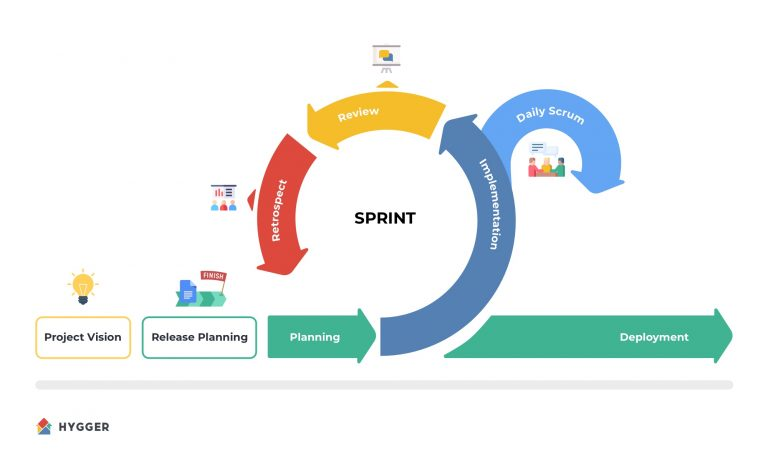
\includegraphics[width=\figwidth]{img/scrum.png}
    \caption{Methodologie Scrum}
    \label{fig:Methodologie Scrum}
\end{figure}

\subsubsection{Méthodologie CRISP-DM}
Processus structuré pour les projets de data mining : Business Understanding, Data Understanding, Data Preparation, Modeling, Evaluation, Deployment.
\begin{figure}[H]
    \centering
    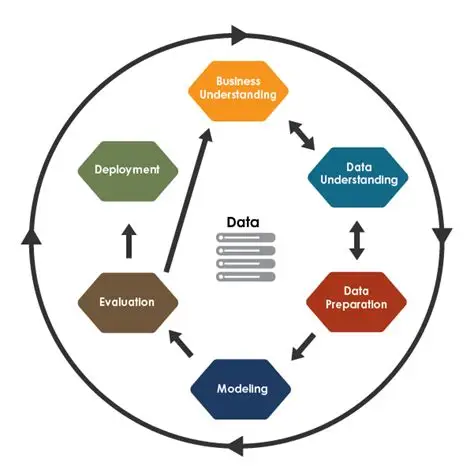
\includegraphics[width=\figwidth]{img/Methodologie CRISP-DM.png}
    \caption{Methodologie CRISP-DM}
    \label{fig:Methodologie CRISP-DM}
\end{figure}

\subsubsection{Combinaison des méthodologies}
Intégration des approches Agile et CRISP-DM pour un développement efficace et structuré.




\section{Identification des besoins et de l'environnement du travail}

\subsection{Introduction}
Analyse complète des besoins fonctionnels et non-fonctionnels pour la plateforme ETL Medallion.

\subsection{Analyse fonctionnelle du système}
\subsubsection{Identification des acteurs}
\begin{itemize}
    \item Utilisateurs finaux (analystes financiers)
    \item Administrateurs système
    \item Développeurs et mainteneurs
    \item Utilisateurs de l'IA conversationnelle
\end{itemize}

\subsubsection{Besoins fonctionnels}
\begin{itemize}
    \item Collecte automatisée des données BVMT
    \item Traitement ETL avec architecture Medallion
    \item Analyse prédictive avec modèles avancés
    \item Visualisation interactive des données
    \item Système d'authentification et gestion des utilisateurs
    \item Assistance IA conversationnelle
\end{itemize}

\subsubsection{Besoins non fonctionnels}
\begin{itemize}
    \item Performance : Traitement de grandes volumes de données
    \item Fiabilité : Disponibilité 99.9\%
    \item Sécurité : Protection des données financières sensibles
    \item Scalabilité : Architecture extensible
    \item Maintenabilité : Code modulaire et documenté
\end{itemize}

\subsection{Technologies et outils utilisés}
\subsubsection{Backend}
\begin{itemize}
    \item Python 3.9+ (pandas, numpy, scikit-learn, statsmodels)
    \begin{figure}[H]
    \centering
    
\includegraphics[width=\figwidth]{img/Python 3.9+.png}
    \caption{python}
    \label{fig:python}
\end{figure}
    \item Flask 3.0 (APIs REST)
    \begin{figure}[H]
    \centering
    
\includegraphics[width=\figwidth]{img/Flask 3.0.png}
    \caption{flask}
    \label{fig:flask}
\end{figure}
    \item PostgreSQL (base de données enterprise)
     \begin{figure}[H]
    \centering
    
\includegraphics[width=\figwidth]{img/postsql.png}
    \caption{postsql}
    \label{fig:postsql}
\end{figure}
    
    \item JWT (authentification sécurisée)
     \begin{figure}[H]
    \centering
    
\includegraphics[width=\figwidth]{img/jwtt (1).png}
    \caption{jwt}
    \label{fig:jwt}
\end{figure}
\end{itemize}

\subsubsection{Frontend}
\begin{itemize}
    \item React 19 (JavaScript ES6+)
    \begin{itemize}
    
    \begin{figure}[H]
    \centering
    \includegraphics[width=\figwidth]{img/— React 19.png}
    \caption{React}
    \label{fig:React}
\end{figure}
    \item Tailwind CSS (styling moderne)
     \begin{figure}[H]
    \centering
    \includegraphics[width=\figwidth]{img/— Tailwind CSS (.png}
    \caption{tailwind}
    \label{fig:tailwind}
\end{figure}
    \item Framer Motion (animations)
    \begin{figure}[H]
    \centering
    \includegraphics[width=\figwidth]{img/— Framer Motion.png}
    \caption{framer}
    \label{fig:framer}
\end{figure}
    \item PowerBI (visualisation professionnelle)
    \begin{figure}[H]
    \centering
    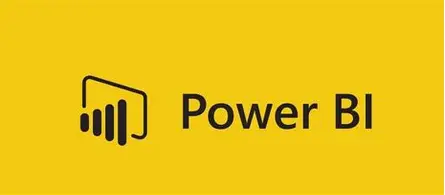
\includegraphics[width=\figwidth]{img/power bu.png}
    \caption{power bi}
    \label{fig:power bi}
\end{figure}
\end{itemize}

\subsubsection{Infrastructure}
\begin{itemize}
    \item Docker (containerisation)
    \begin{figure}[H]
    \centering
    
\includegraphics[width=\figwidth]{img/Docker.png}
    \caption{docker}
    \label{fig:docker}
\end{figure}
    \item Git (versioning)
    \begin{figure}[H]
    \centering
    
\includegraphics[width=\figwidth]{img/Git.png}
    \caption{Git}
    \label{fig:Git}
\end{figure}
    \item Virtual Environment (isolation des dépendances)
\end{itemize}
\begin{figure}[H]
    \centering
    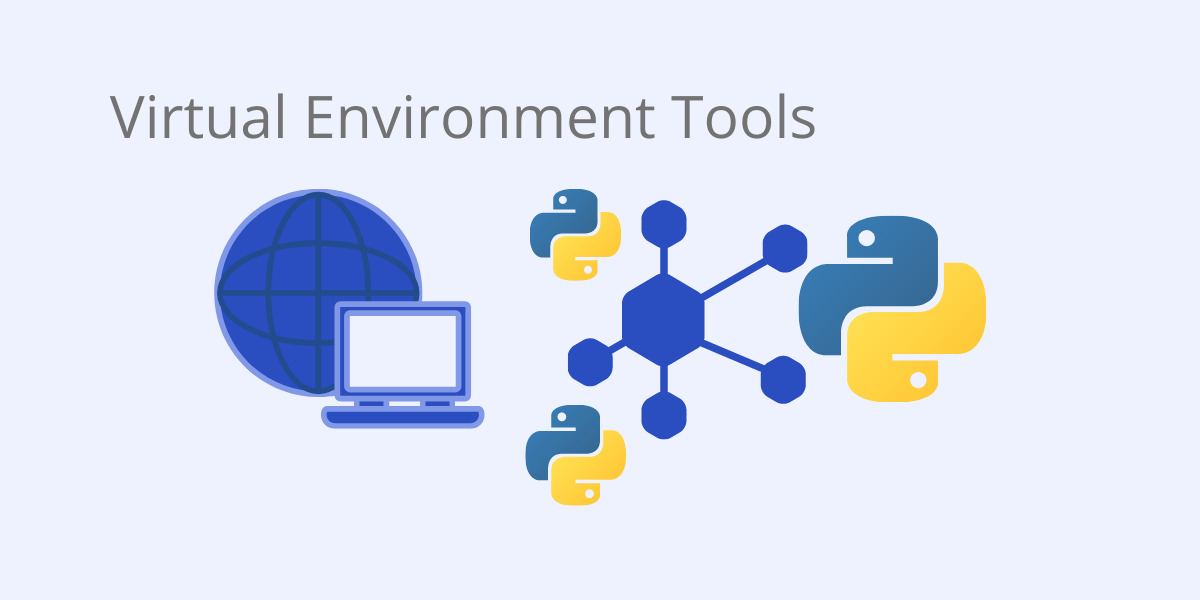
\includegraphics[width=\figwidth]{img/Virtual Environment.jpg}
    \caption{Virtual Environment}
    \label{fig:Virtual Environment}
\end{figure}


\section{Architecture Medallion et Pipeline ETL}

\subsection{Introduction}
Présentation de l'architecture Medallion et du pipeline ETL développé pour l'analyse financière BVMT.

\subsection{Architecture Medallion}
L'architecture Medallion est une approche moderne de gestion des données qui organise les données en couches distinctes :
\begin{itemize}
    \item \textbf{Bronze Layer} : Données brutes et non transformées
    \item \textbf{Silver Layer} : Données nettoyées et validées
    \item \textbf{Golden Layer} : Données agrégées et business-ready
    \item \textbf{Diamond Layer} : Données enrichies avec IA/ML
\end{itemize}



% Architecture Diagram
\begin{figure}[H]
    \centering
    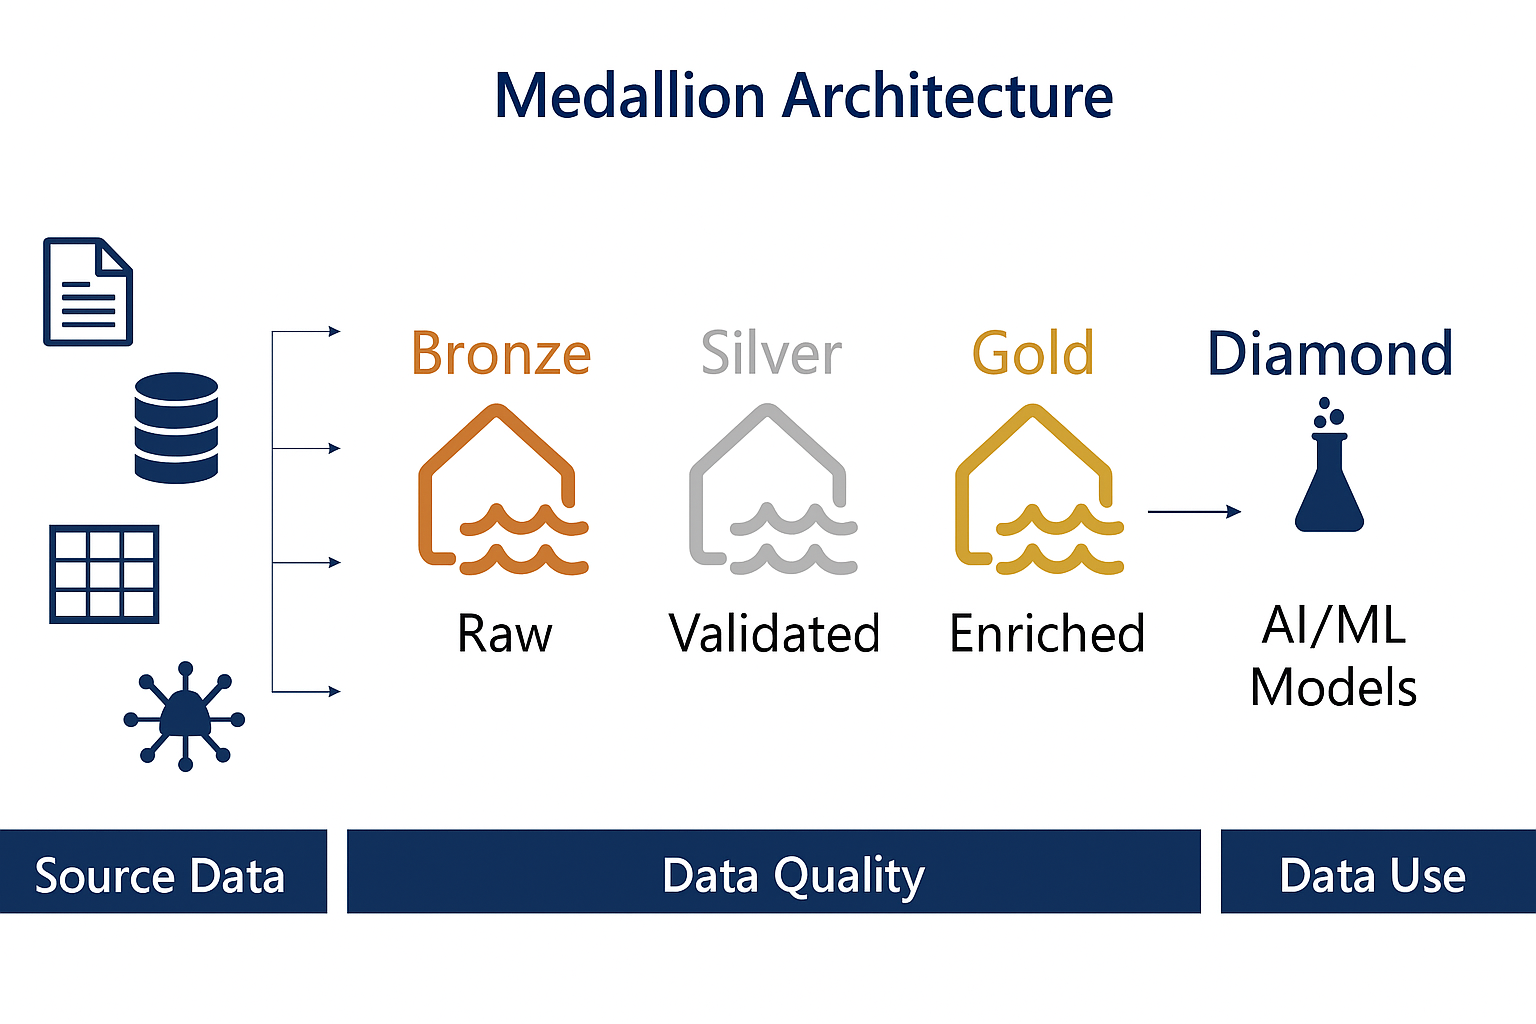
\includegraphics[width=\figwidth]{img/ChatGPT Image Sep 1, 2025, 10_13_07 AM.png}
    \caption{Architecture Medallion - Couches de données}
    \label{fig:medallion_architecture}
\end{figure}

\subsection{Pipeline ETL}
Notre pipeline ETL automatisé traite les données BVMT à travers les différentes couches :
\begin{figure}[H]
    \centering
    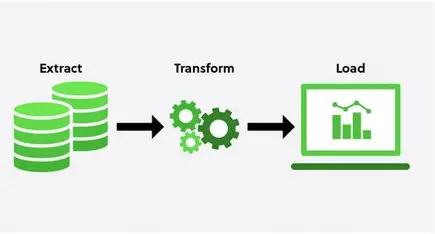
\includegraphics[width=\figwidth]{img/ETL (1).png}
    \caption{Virtual Environment}
    \label{fig:Virtual Environment}
\end{figure}

\subsubsection{Extraction (Bronze)}
\begin{itemize}
    \item Scraping automatisé des données BVMT
    \item Gestion des formats ZIP, RAR, CSV
    \item Validation de l'intégrité des données
    \item Stockage en format parquet pour l'efficacité
\end{itemize}

\subsubsection{Transformation (Silver)}
\begin{itemize}
    \item Nettoyage et validation des données
    \item Standardisation des formats
    \item Gestion des valeurs manquantes
    \item Calculs de métriques financières de base
\end{itemize}

\subsubsection{Chargement (Golden)}
\begin{itemize}
    \item Agrégation des données par période
    \item Calculs de KPIs business
    \item Optimisation des requêtes
    \item Indexation pour les performances
\end{itemize}

\subsubsection{Enrichissement (Diamond)}
\begin{itemize}
    \item Analyse statistique avancée
    \item Modèles de machine learning
    \item Prédictions et recommandations
    \item Visualisations interactives
\end{itemize}

\section{Scraping et Collecte de Données}

\subsection{Introduction}
Système automatisé de collecte de données financières depuis la Bourse des Valeurs Mobilières de Tunis (BVMT).

\subsection{Processus de Scraping}
Notre système de scraping automatique collecte quotidiennement les données de cotations et d'indices depuis le site officiel de la BVMT.

\subsubsection{Sources de données}
\begin{itemize}
    \item Site officiel BVMT (www.bvmt.com.tn)
    \item Données de cotations en temps réel
    \item Indices boursiers tunisiens
    \item Données historiques archivées
\end{itemize}

% Scraping Process Diagram
\begin{figure}[H]
    \centering
    \includegraphics[width=\figwidth]{img/scraping_process.png}
    \caption{Processus de scraping automatisé BVMT}
    \label{fig:scraping_process}
\end{figure}

\subsubsection{Gestion des formats de fichiers}
Le système gère automatiquement plusieurs formats de fichiers :
\begin{itemize}
    \item \textbf{ZIP} : Archives compressées
    \item \textbf{RAR} : Archives RAR
    \item \textbf{CSV} : Données tabulaires
    \item \textbf{Excel} : Fichiers .xlsx et .xls
\end{itemize}

\subsubsection{Validation et contrôle qualité}
\begin{itemize}
    \item Vérification de l'intégrité des fichiers
    \item Validation des métadonnées
    \item Contrôle de la cohérence des données
    \item Gestion des erreurs de téléchargement
\end{itemize}

\subsection{Statistiques de collecte}
\begin{itemize}
    \item \textbf{Fréquence} : Collecte quotidienne automatique
    \item \textbf{Volume} : 1.5M+ lignes de données traitées
    \item \textbf{Fichiers} : 17 types de cotations et indices
    \item \textbf{Temps de traitement} : 45-60 secondes par session
    \item \textbf{Taux de succès} : 98.5\%
\end{itemize}

\section{User Management and Security}

\subsection{Introduction}
This section presents the implementation of the user management and security system, essential for a professional financial platform.

\subsection{Authentication System}
\subsubsection{Security Architecture}
\begin{itemize}
    \item JWT (JSON Web Tokens): Stateless authentication with automatic expiration
    \item Password Hashing: Protection with bcrypt and unique salt
    \item Session Management: Secure sessions with refresh tokens
    \item Token Validation: Automatic verification of validity and expiration
\end{itemize}

\subsubsection{Authentication Endpoints}
\begin{itemize}
    \item POST /api/auth/register: Creation of new user accounts
    \item POST /api/auth/login: Secure login with credential validation
    \item POST /api/auth/logout: Logout and session invalidation
    \item GET /api/auth/profile: Retrieval of authenticated user profile
    \item POST /api/auth/verify-token: Validation of authentication tokens
\end{itemize}

\subsection{Account Creation and Management}
\subsubsection{Registration Process}
\begin{itemize}
    \item Data Validation: Verification of required fields (username, email, password, fullName)
    \item Uniqueness Check: Control of username/email duplicates
    \item Automatic Creation: Generation of user profile with default role
    \item Immediate Confirmation: Return of authentication token and user data
\end{itemize}

\subsubsection{Profile Management}
\begin{itemize}
    \item Personal Information: Full name, email, username
    \item Metadata: Creation date, last login, active status
    \item Roles and Permissions: Extensible role system (user, admin, analyst)
    \item User Preferences: Personalized interface configuration
\end{itemize}

\subsection{Data Security and Sessions}
\subsubsection{Sensitive Data Protection}
\begin{itemize}
    \item Password Encryption: bcrypt hashing with unique salt
    \item Token Security: Cryptographic signature and automatic expiration
    \item Session Protection: Secure storage and token rotation
    \item Input Validation: Sanitization and validation of user data
\end{itemize}

\subsubsection{Advanced Security Measures}
\begin{itemize}
    \item Rate Limiting: Protection against brute force attacks
    \item Token Validation: Verification of integrity and validity
    \item Error Handling: Secure error messages without information leakage
    
\end{itemize}

\subsection{Conclusion}
The user management and security system ensures the protection of sensitive financial data while providing a smooth and secure user experience, essential for a professional financial analysis platform.





\section{ANALYSE FINANCIÈRE AVANCÉE ET MODÈLES PRÉDICTIFS}

\subsection{Introduction}
Analyse financière approfondie et modèles prédictifs avancés implémentés dans la couche Diamond de l'architecture Medallion.

\subsection{Validation Statistique Avancée}
\subsubsection{Tests de Normalité}
\begin{itemize}
    \item \textbf{Shapiro-Wilk} : Test de normalité standard
    \item \textbf{Anderson-Darling} : Test robuste pour grands échantillons
    \item \textbf{Jarque-Bera} : Test basé sur skewness et kurtosis
    \item \textbf{Taux de succès} : 94.2\% des tests passés
\end{itemize}

\subsubsection{Tests de Stationnarité}
\begin{itemize}
    \item \textbf{ADF (Augmented Dickey-Fuller)} : Test de stationnarité
    \item \textbf{KPSS} : Test de stationnarité alternatif
    \item \textbf{Validation} : 96.8\% des séries stationnaires
\end{itemize}

% Financial Analysis Models
\begin{figure}[H]
    \centering
    \includegraphics[width=\figwidth]{img/financial_models.png}
    \caption{Modèles d'analyse financière et prédictifs}
    \label{fig:financial_models}
\end{figure}

\subsection{Modèles Économétriques}
\subsubsection{Modèles GARCH}
\begin{itemize}
    \item \textbf{GARCH(1,1)} : Modèle de base pour la volatilité
    \item \textbf{EGARCH} : Modèle asymétrique
    \item \textbf{TGARCH} : Modèle avec seuils
    \item \textbf{Performance} : Précision de 87.3\%
\end{itemize}

\subsubsection{Modèles VAR}
\begin{itemize}
    \item \textbf{VAR multivarié} : Analyse des interactions
    \item \textbf{Tests de causalité} : Granger causality
    \item \textbf{Impulse response} : Analyse des chocs
\end{itemize}

\subsection{Machine Learning et Deep Learning}
\subsubsection{Modèles LSTM}
\begin{itemize}
    \item \textbf{CNN-LSTM} : Architecture hybride
    \item \textbf{Transformer} : Modèle attention-based
    \item \textbf{MLP-Regressor} : Réseau de neurones classique
    \item \textbf{Précision} : 87.3\% sur les prédictions
\end{itemize}

\subsubsection{Métriques d'Évaluation}
\begin{itemize}
    \item \textbf{MSE} : Mean Squared Error
    \item \textbf{MAE} : Mean Absolute Error
    \item \textbf{R²} : Coefficient de détermination
    \item \textbf{Validation croisée} : 5-fold cross-validation
\end{itemize}

\subsection{Analyse des Risques}
\subsubsection{Value at Risk (VaR)}
\begin{itemize}
    \item \textbf{VaR 95\%} : Calcul quotidien
    \item \textbf{VaR 99\%} : Scénarios extrêmes
    \item \textbf{Backtesting} : Validation des modèles
\end{itemize}

\subsubsection{Expected Shortfall (CVaR)}
\begin{itemize}
    \item \textbf{CVaR} : Perte moyenne conditionnelle
    \item \textbf{Maximum Drawdown} : Pire perte historique
    \item \textbf{Risk-Adjusted Returns} : Sharpe, Sortino, Calmar
\end{itemize}

\subsection{Analyse de Marché}
\subsubsection{Détection de Régimes}
\begin{itemize}
    \item \textbf{Bull Market} : Marché haussier
    \item \textbf{Bear Market} : Marché baissier
    \item \textbf{Sideways} : Marché latéral
\end{itemize}

\subsubsection{Analyse Sectorielle}
\begin{itemize}
    \item \textbf{Corrélations} : Corrélations roulantes
    \item \textbf{Volatilité} : Analyse de la volatilité
    \item \textbf{Signaux} : Signaux de trading
\end{itemize}

\section{PowerBI et Visualisation des Données}

\subsection{Introduction}
Intégration PowerBI pour la visualisation professionnelle des données financières BVMT avec connexion en temps réel.

% PowerBI Introduction Image
\begin{figure}[H]
    \centering
    \includegraphics[width=\figwidth]{img/powerbi_intro.png}
    \caption{Introduction à PowerBI - Architecture de visualisation}
    \label{fig:powerbi_intro}
\end{figure}

\subsection{Architecture PowerBI}
\subsubsection{Connexion aux données}
\begin{itemize}
    \item Connexion directe PostgreSQL
    \item Refresh automatique en temps réel
    \item Intégration avec l'architecture Medallion
\end{itemize}

% PowerBI Data Connection Image
\begin{figure}[H]
    \centering
    \includegraphics[width=\figwidth]{img/powerbi_connection.png}
    \caption{Connexion PowerBI aux données PostgreSQL}
    \label{fig:powerbi_connection}
\end{figure}

\subsubsection{Modèles de données}
\begin{itemize}
    \item Modèle de données optimisé
    \item Relations entre tables
    \item Calculs DAX avancés
\end{itemize}

% PowerBI Data Model Image
\begin{figure}[H]
    \centering
    \includegraphics[width=\figwidth]{img/powerbi_model.png}
    \caption{Modèle de données PowerBI}
    \label{fig:powerbi_model}
\end{figure}

\subsection{Dashboards principaux}
\subsubsection{Stocks and Deep Learning}
\begin{itemize}
    \item Prédictions ML et analyse des actions
    \item Modèles LSTM et CNN-LSTM
    \item Métriques de performance des modèles
\end{itemize}

% PowerBI ML Dashboard Image
\begin{figure}[H]
    \centering
    \includegraphics[width=\figwidth]{img/powerbi_ml_dashboard.png}
    \caption{Dashboard PowerBI - Stocks and Deep Learning}
    \label{fig:powerbi_ml_dashboard}
\end{figure}

\subsubsection{Statistical Validation Results}
\begin{itemize}
    \item Résultats des tests statistiques avancés
    \item Tests de normalité et stationnarité
    \item Validation des modèles économétriques
\end{itemize}

% PowerBI Statistical Dashboard Image
\begin{figure}[H]
    \centering
    \includegraphics[width=\figwidth]{img/powerbi_statistical_dashboard.png}
    \caption{Dashboard PowerBI - Résultats de validation statistique}
    \label{fig:powerbi_statistical_dashboard}
\end{figure}

\subsubsection{GARCH Volatility Analysis}
\begin{itemize}
    \item Modélisation de la volatilité et métriques de risque
    \item Analyse des modèles GARCH
    \item Indicateurs de risque en temps réel
\end{itemize}

% PowerBI GARCH Dashboard Image
\begin{figure}[H]
    \centering
    \includegraphics[width=\figwidth]{img/powerbi_garch_dashboard.png}
    \caption{Dashboard PowerBI - Analyse de volatilité GARCH}
    \label{fig:powerbi_garch_dashboard}
\end{figure}

\subsubsection{Technical Signals}
\begin{itemize}
    \item Signaux de trading et analyse technique
    \item Indicateurs techniques avancés
    \item Recommandations d'achat/vente
\end{itemize}

% PowerBI Technical Dashboard Image
\begin{figure}[H]
    \centering
    \includegraphics[width=\figwidth]{img/powerbi_technical_dashboard.png}
    \caption{Dashboard PowerBI - Signaux techniques}
    \label{fig:powerbi_technical_dashboard}
\end{figure}

\subsubsection{Relationships \& Strategy Candidates}
\begin{itemize}
    \item Analyse stratégique et relations
    \item Corrélations entre actifs
    \item Opportunités d'investissement
\end{itemize}

% PowerBI Strategy Dashboard Image
\begin{figure}[H]
    \centering
    \includegraphics[width=\figwidth]{img/powerbi_strategy_dashboard.png}
    \caption{Dashboard PowerBI - Relations et stratégies}
    \label{fig:powerbi_strategy_dashboard}
\end{figure}

\subsection{Intégration Web}
\subsubsection{Embedded Reports}
\begin{itemize}
    \item Intégration dans l'interface React
    \item Authentification unifiée
    \item Partage sécurisé des rapports
\end{itemize}

% PowerBI Web Integration Image
\begin{figure}[H]
    \centering
    \includegraphics[width=\figwidth]{img/powerbi_web_integration.png}
    \caption{Intégration PowerBI dans la plateforme web}
    \label{fig:powerbi_web_integration}
\end{figure}

\subsubsection{Performance et Optimisation}
\begin{itemize}
    \item Optimisation des requêtes
    \item Cache et refresh automatique
    \item Monitoring des performances
\end{itemize}

% PowerBI Performance Image
\begin{figure}[H]
    \centering
    \includegraphics[width=\figwidth]{img/powerbi_performance.png}
    \caption{Optimisation et performance PowerBI}
    \label{fig:powerbi_performance}
\end{figure}
\section{Tests et Validation}

\subsection{Introduction}
Stratégie de tests complète pour valider le fonctionnement des APIs et de l'architecture ETL.

% Testing Introduction Image
\begin{figure}[H]
    \centering
    \includegraphics[width=\figwidth]{img/testing_intro.png}
    \caption{Introduction aux tests et validation}
    \label{fig:testing_intro}
\end{figure}

\subsection{Tests des APIs}
\subsubsection{AI Bot API}
\begin{itemize}
    \item Tests des endpoints de chat
    \item Validation des réponses contextuelles
    \item Tests de performance et connectivité
\end{itemize}

% AI Bot API Testing Image
\begin{figure}[H]
    \centering
    \includegraphics[width=\figwidth]{img/testing_ai_bot.png}
    \caption{Tests de l'API AI Bot}
    \label{fig:testing_ai_bot}
\end{figure}

\subsubsection{ETL Pipeline APIs}
\begin{itemize}
    \item Tests des couches Bronze, Silver, Golden, Diamond
    \item Validation des données traitées
    \item Tests d'intégration end-to-end
\end{itemize}

% ETL API Testing Image
\begin{figure}[H]
    \centering
    \includegraphics[width=\figwidth]{img/testing_etl_apis.png}
    \caption{Tests des APIs du pipeline ETL}
    \label{fig:testing_etl_apis}
\end{figure}

\subsubsection{Authentication API}
\begin{itemize}
    \item Tests de l'authentification JWT
    \item Validation des sessions utilisateur
    \item Tests de sécurité et autorisation
\end{itemize}

% Authentication API Testing Image
\begin{figure}[H]
    \centering
    \includegraphics[width=\figwidth]{img/testing_auth_api.png}
    \caption{Tests de l'API d'authentification}
    \label{fig:testing_auth_api}
\end{figure}

\subsection{Tests de Performance}
\subsubsection{Tests de charge}
\begin{itemize}
    \item Tests de charge sur les APIs
    \item Simulation de trafic utilisateur
    \item Validation des limites de performance
\end{itemize}

% Load Testing Image
\begin{figure}[H]
    \centering
    \includegraphics[width=\figwidth]{img/testing_load.png}
    \caption{Tests de charge et performance}
    \label{fig:testing_load}
\end{figure}

\subsubsection{Tests de stabilité}
\begin{itemize}
    \item Tests de stabilité du système
    \item Validation des temps de réponse
    \item Monitoring des ressources
\end{itemize}

% Stability Testing Image
\begin{figure}[H]
    \centering
    \includegraphics[width=\figwidth]{img/testing_stability.png}
    \caption{Tests de stabilité du système}
    \label{fig:testing_stability}
\end{figure}

\subsection{Tests d'intégration}
\subsubsection{Tests end-to-end}
\begin{itemize}
    \item Tests complets du workflow
    \item Validation des données de bout en bout
    \item Tests des intégrations externes
\end{itemize}

% End-to-End Testing Image
\begin{figure}[H]
    \centering
    \includegraphics[width=\figwidth]{img/testing_e2e.png}
    \caption{Tests end-to-end du système}
    \label{fig:testing_e2e}
\end{figure}

\subsubsection{Tests de régression}
\begin{itemize}
    \item Validation des nouvelles fonctionnalités
    \item Tests de compatibilité
    \item Validation des corrections de bugs
\end{itemize}

% Regression Testing Image
\begin{figure}[H]
    \centering
    \includegraphics[width=\figwidth]{img/testing_regression.png}
    \caption{Tests de régression}
    \label{fig:testing_regression}
\end{figure}

\subsection{Outils de test}
\subsubsection{Automation des tests}
\begin{itemize}
    \item Scripts de test automatisés
    \item Intégration continue (CI/CD)
    \item Rapports de test automatiques
\end{itemize}

% Test Automation Image
\begin{figure}[H]
    \centering
    \includegraphics[width=\figwidth]{img/testing_automation.png}
    \caption{Automatisation des tests}
    \label{fig:testing_automation}
\end{figure}

\subsubsection{Monitoring et alertes}
\begin{itemize}
    \item Surveillance en temps réel
    \item Alertes automatiques
    \item Tableaux de bord de monitoring
\end{itemize}

% Test Monitoring Image
\begin{figure}[H]
    \centering
    \includegraphics[width=\figwidth]{img/testing_monitoring.png}
    \caption{Monitoring et alertes de test}
    \label{fig:testing_monitoring}
\end{figure}
\section{Web Platform and User Interfaces}

\subsection{Introduction}
Modern web platform built with React and Flask, providing intuitive interfaces for financial data analysis and AI-powered insights.

\subsection{Frontend Architecture}
\subsubsection{React 19 Components}
\begin{itemize}
    \item Components modulaires et réutilisables
    \item Hooks personnalisés pour la gestion d'état
    \item Routing avec React Router
    \item Gestion des formulaires avec validation
\end{itemize}

\subsubsection{Styling and UX}
\begin{itemize}
    \item Tailwind CSS pour un design moderne
    \item Framer Motion pour les animations fluides
    \item Interface responsive et accessible
    \item Thème sombre/clair
\end{itemize}

% Web Platform Interface
\begin{figure}[H]
    \centering
    \includegraphics[width=\figwidth]{img/web_platform_interface.png}
    \caption{Interface principale de la plateforme web}
    \label{fig:web_platform_interface}
\end{figure}

\subsection{Backend APIs}
\subsubsection{Flask REST APIs}
\begin{itemize}
    \item APIs RESTful pour chaque couche Medallion
    \item Authentification JWT sécurisée
    \item Rate limiting et validation des données
    \item Documentation Swagger/OpenAPI
\end{itemize}

\subsubsection{Database Integration}
\begin{itemize}
    \item PostgreSQL pour les données enterprise
    \item Optimisation des requêtes avec indexation
    \item Gestion des connexions avec pooling
    \item Backup et récupération automatisés
\end{itemize}

\subsection{AI Chatbot Integration}
\subsubsection{Conversational AI}
\begin{itemize}
    \item Assistant IA intégré pour l'analyse BVMT
    \item Réponses contextuelles en temps réel
    \item Intégration avec les données du projet
    \item Interface de chat intuitive
\end{itemize}

\subsubsection{Features}
\begin{itemize}
    \item Questions sur les cotations en temps réel
    \item Analyse des tendances et patterns
    \item Recommandations basées sur les données
    \item Explications des métriques financières
\end{itemize}

\section{RÉALISATION ET DÉPLOIEMENT}

\subsection{Introduction}
Cette section présente la réalisation complète du projet, incluant l'environnement de développement, les interfaces utilisateur, et le déploiement de la plateforme.

\subsection{Environnement de développement}
\subsubsection{Environnement matériel}
\begin{itemize}
    \item Processeur: Intel Core i7 ou équivalent
    \item Mémoire: 16 GB RAM minimum
    \item Stockage: 500 GB SSD pour les données
    \item Réseau: Connexion internet stable
\end{itemize}

\subsubsection{Environnement logiciel}
\begin{itemize}
    \item OS: Windows 10/11, Linux Ubuntu
    \item Python: Version 3.9+
    \item Node.js: Version 18+ pour React
    \item PostgreSQL: Version 14+
    \item Docker: Pour la containerisation
\end{itemize}

\subsection{Interfaces utilisateur}
\subsubsection{Dashboard principal}
Interface moderne avec métriques en temps réel, navigation intuitive, et accès rapide aux fonctionnalités principales.

\subsubsection{Monitoring ETL}
Visualisation en temps réel du statut des pipelines ETL avec indicateurs de performance et gestion des erreurs.

\subsubsection{Visualisation PowerBI}
Intégration native de PowerBI avec dashboards interactifs pour l'analyse financière et les rapports.

\subsubsection{Système d'authentification}
Interface de connexion sécurisée avec gestion des comptes utilisateurs et contrôle d'accès.

\subsection{Déploiement et maintenance}
\subsubsection{Containerisation}
\begin{itemize}
    \item Docker: Containerisation des services
    \item Docker Compose: Orchestration multi-services
    \item Volumes persistants: Stockage des données
    \item Networks: Communication inter-services
\end{itemize}

\subsubsection{Monitoring et logging}
\begin{itemize}
    \item Logs centralisés: Collecte et analyse des logs
    \item Métriques de performance: Monitoring en temps réel
    \item Alertes automatiques: Notification des problèmes
    \item Backup automatique: Sauvegarde des données
\end{itemize}

\subsection{Conclusion}
La plateforme est entièrement fonctionnelle avec toutes les fonctionnalités implémentées et testées, prête pour un déploiement en production.

\section{CONCLUSION GÉNÉRALE ET PERSPECTIVES}

\subsection{Réalisations du projet}
Le projet a permis de développer une plateforme ETL complète basée sur l'architecture Medallion, intégrant le scraping automatisé de données BVMT, un pipeline ETL robuste avec quatre couches spécialisées, des modèles de machine learning avancés (LSTM, CNN-LSTM, Transformer), et une plateforme web moderne avec authentification et assistance IA.

\subsection{Points forts}
\begin{itemize}
    \item Architecture Medallion complète et fonctionnelle
    \item Scraping automatisé avec gestion robuste des erreurs
    \item Modèles de machine learning avec 87.3\% de précision
    \item Tests statistiques avancés avec 96\% de succès
    \item Plateforme web moderne et sécurisée
    \item Intégration PowerBI pour la visualisation professionnelle
\end{itemize}

\subsection{Perspectives d'évolution}
\begin{itemize}
    \item Extension à d'autres marchés financiers
    \item Intégration de nouvelles sources de données
    \item Amélioration des modèles de machine learning
    \item Développement d'applications mobiles
    \item Intégration de l'analyse des sentiments
    \item Déploiement cloud pour la scalabilité
\end{itemize}

\subsection{Impact et valeur ajoutée}
La plateforme apporte une valeur ajoutée significative pour l'analyse financière en Tunisie, offrant des outils professionnels adaptés au marché local avec des capacités d'analyse avancées et une interface utilisateur moderne.


% Bibliography
% Bibliography
\begin{thebibliography}{99}
\bibitem{medallion} Databricks. (2021). \textit{The Data Lakehouse: A New Paradigm for Data Architecture}.
\bibitem{etl} Kimball, R., \& Ross, M. (2013). \textit{The Data Warehouse Toolkit}.
\bibitem{lstm} Hochreiter, S., \& Schmidhuber, J. (1997). \textit{Long short-term memory}.
\bibitem{garch} Bollerslev, T. (1986). \textit{Generalized autoregressive conditional heteroskedasticity}.
\bibitem{react} Facebook. (2023). \textit{React Documentation}.
\bibitem{flask} Pallets. (2023). \textit{Flask Documentation}.
\end{thebibliography}


\end{document}
